\documentclass[11pt,a4paper]{report}
\usepackage[utf8]{inputenc}
\usepackage{amsmath}
\usepackage{amsfonts}
\usepackage{amssymb}
\usepackage{graphicx}
\author{Jan Dziedzic}
\usepackage{fancyhdr}
\usepackage{float}
\usepackage[section]{placeins}
\title{PycMan}
\fancypagestyle{}{%
\fancyhf{} % clear all header and footer fields
\fancyhead[RE,LO]{\chaptername \thechapter}
\renewcommand{\headrulewidth}{0pt}
\renewcommand{\footrulewidth}{0pt}
\renewcommand{\chaptername}{Part}}
\newcommand{\dsubsection}[1]{\FloatBarrier \subsection{'#1'}}
\newenvironment{img}{
	\begin{center}
		\begin{figure}[H]
			\begin{center}
			
}{
	\end{center}
		\end{figure}
			\end{center}
}

\usepackage{listings}
\usepackage{color}

\definecolor{codegreen}{rgb}{0,0.6,0}
\definecolor{codegray}{rgb}{0.5,0.5,0.5}
\definecolor{codepurple}{rgb}{0.58,0,0.82}
\definecolor{backcolour}{rgb}{0.95,0.95,0.92}

\lstdefinestyle{mystyle}{
	backgroundcolor=\color{backcolour},   
	commentstyle=\color{codegreen},
	keywordstyle=\color{magenta},
	numberstyle=\tiny\color{codegray},
	stringstyle=\color{codepurple},
	basicstyle=\footnotesize,
	breakatwhitespace=false,         
	breaklines=true,                 
	captionpos=b,                    
	keepspaces=true,                 
	numbers=left,                    
	numbersep=5pt,                  
	showspaces=false,                
	showstringspaces=false,
	showtabs=false,                  
	tabsize=2
}

\lstset{style=mystyle}




\begin{document}
	\maketitle
	\newpage
	\thispagestyle{empty}
	$$$$
	\newpage
	\thispagestyle{empty}
	\tableofcontents
	\chapter{Project Definition and Analysis}
		\newpage
		\section{Project Definition}
		
			\begin{img}
			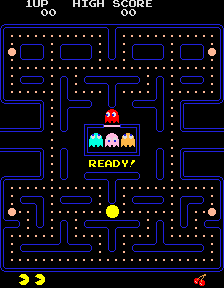
\includegraphics{images/1_1}\\
			\caption{Original Pac-Man screen. Source is Reference \ref{stronaopacmanie}.}
			\label{oryg_pacman}
			\end{img}
		
			As my project, I have decided to present a game written in Python, based around one of its modules - pygame. As I have not had as much time to prepare my project as my colleagues, I have decided that the concept of the game must be simple, yet allowing to demonstrate my programming and computational thinking skills. For this purpose I have decided to mimic the iconic PacMan game.
			For picture of the original game screen please refer to Figure \ref{oryg_pacman}
			
			
		
			Called PycMan (utilizing the fact that many of Python modules have a prefix 'py' in their name), the game itself strongly resembles the original, yet with some meaningful changes. Like in the original - player can move in four directions (left, right, up and down), collecting coins and avoiding ghosts.
			
			
			The game develops critical thinking skills and takes effect of human nature of taking risks and tackling unknown - with having more confidence when predicting ghost behavior, the player actually gets better when playing despite problems generally low complexity.
			
			Actually the game itself may be referred as to playing tag in a transparent maze. Such a play would be very hard for a human to enjoy as analyzing transparent walls while running and predicting opponent's next move is a far too complex problem for human cognition. That's why computational approach on this game is required - where player can see ghosts from above the board whilst ghost may exhibit algorithmically advanced behavior.
		\section{Stakeholders}
			Proposed end user group is really wide. As the game itself can be launched on virtually any device due to Python versatility, it may be used on a spectrum of devices with different controllers, from mobile phones and smart watches through PCs reaching as far as game console emulators mimicking the most authentic PacMan game experience. Such portability should satisfy most users.
			
			The game should grab attention of children - with small challenges that don't require complex thinking and rather promote manual skills and reflex; those who seek quick brainteaser whilst attempting to play with more focus on tactics of ghost avoidance and finally, old gamers who played original PacMan but now they might want to try more modern version with a different approach to critical game mechanisms.
		\section{Software Challenges}
			All software used to develop the game but is not necessarily required to run it:
			\begin{itemize}
				\item Python3
				\subitem Pillow module
				\subitem Pygame module
				\item Pycharm Professional
				\item GIMP - GNU Image Manipulation Program
				\item \LaTeX
				\item TeXstudio
			\end{itemize}
			
			The greatest advantage that convinced me to actually use Python for my game was its portability. As an interpretable programming language, the code of the game remains universal throughout different operating systems and processor architectures. My decision was also influenced by my previous experience with this language and my desire to actually get better around it. It's also free, meaning that everyone can take benefit of my game, without having to buy a license from a third party.
			
			Also, whilst most of my experience was with Python2 I have decided that it's the right time to move on and actually start using Python3, which is reportedly faster and offers more functionality while providing greater stability.
			
			Still, Python does not offer the speed one may expect from a programming language suitable for complex games. Advanced non-optimal solutions need to be thought of and substituted with faster algorithms in order for the game to run smooth on machines lacking processing power.
			
			Happily Python is an objective language - which greatly helped with some designs.
			
			As it's also an interpretable language, it's way easier to debug as one may actually run every single line of code step by step to see variable values changing. Python interpreters also provide a very generous error descriptions greatly helping with bug fixing. 
			
			The closest I could get with Python to making a full featured game conveniently was to use pygame. It's a rather good module supplying some basic functionality one may expect from assisted-design library for creating 2D games. Some functions were not supported out of the box, like level storing (suitable for my purpose) and loading and these had to be implemented by myself as an addition.
			
			Pygame also doesn't have a tiling system I wanted for level designs, to make my game resemble original PacMan in terms of design. I had to write such myself. A similar situation occurred when I wanted to implement discrete "Time Segments" (see Section \ref{timesegments} for reference). For a game such as PacMan I find such solutions to be a very useful optimization and yet these are missing from the pygame module.
			
			Pycharm by JetBrains was used as a Python IDE - it is a really convinient solution and comes with a lot of useful features. It was chosen due to my previous positive experience with it.
			
			GIMP was used to produce graphics resources of the game as well as levels - described later. I found it to be a great deal of overkill for such basic tasks but I am very familiar with it's interface and tools which were of great help especially during the design of semi-transparent ghost graphics.
			
			\LaTeX and Texstudio were used to develop this document. As I identify as a pro-open-source-software person I wanted to use \LaTeX instead of word processors with a far advanced UI, like Microsoft Word. A practical reason behind this - \LaTeX provides an absolutely full flexibility. And even when it doesn't have a function I might want to use - I can always write such myself.
			
			All development was done on an Ubuntu-running computer, therefore	
			I must proudly admit that during the entire design process no non-free software was used. All software was either opensource, freeware or free for education.
			
		\section{The Interview}
			\label{interview}
			To assess interest and gain insight of the potential market for the game, I have interviewed my fellow schoolmate - Wojciech Wojtkowski on his opinion of my approach to redesigning PacMan.
			
			-Hello Wojciech, may I interest you with my IT project - the PycMan, next generation of the classic PacMan with smarter ghosts and different mechanics?
			
			-Sure mate, go ahead!
			
			-Ok, so these are some concept graphics [first two levels were exhibited]...
			
			-...but it looks just like the original!
			
			-Yes, there is a strong resemblance in terms of the graphics, that's what I am aiming for. The biggest difference is how the ghost work.
			
			-Oh, tell me more.
			
			-So, in the classical PacMan, the ghost have their designated area they launch from, A.K.A. "The Ghost House", I want to get rid of that, instead all ghosts will start from predefined locations different for each level.
			
			-That means they will chase you from the exact beginning of the level, isn't that going to make the game harder?
			
			-Yes it will, that is the goal. But that's not the main change. They will be smarter than the originals.
			
			-You mean that the way they move is going to be less predictable?
			
			-That's true, I want to utilize a rather complex algorithm to make them chase player more efficiently.
			
			-Didn't the original have the most efficient solution?
			
			-No, the target machines lacked processing power and memory in the past to actually use that with the game not slowing down. Now, when newer computers are available, I can actually use that.
			
			-So if they were quite stupid then and the game was still hard, won't making them smart render the game impossible to win?
			
			-That's what I am afraid of, I need to find a way to give the player some advantage. Do you, as an experienced gamer, have any idea how to do that?
			
			-I think that making the ghost chase the player indirectly may be the way, how about them tailing the PycMan?
			
			-Yeah, that migh be fine but this may eventually lead to them not catching it at all if it doesn't move.
			
			-Oh, that might be the case.
			
			-Actually I have one solution in mind - making them a little bit slower than the player.
			
			-Seems okay, thought I think that one may run away from them, do a risky eating-maneuver then and regain the distance lost. Repeating that will make the game easy and very boring actually.
			
			-Oh, true, I will have to think of these solutions. Probably final version will be designed during beta testing based on player satisfaction with each of these methods.
			
			-Good idea to let the players decide. Actually - on the player-decision thing. One thing that I always wanted with PacMan is to design my own levels. Can you make it possible?
			
			-Yeah, I already have a solution in mind that will make it very easy for anyone to design their own maze, if you say that's going to interest players, I will surely include that.
			
			-Cool! Thanks for letting me know, can I play that game later?
			
			-Of course, as soon as I release the beta.
			
			-Perfect, thank you then, I look forward to playing it.
			
			-Thank you for the talk and insight. Bye.
			
			-Bye.
		\section{Requirement specification (success criteria)}
			For the project to succeed the following criteria must be met:\\
			\begin{enumerate}
				\item 
				The game must resemble the original PacMan in terms of graphical design and some of the mechanics.
				\begin{enumerate}
					\item
						Game graphics should be of similar color and shape to the originals.
					\item
						Player sprite is an iconic yellow ball with 'mouth'.
					\item
						Player sprite should rotate with 'mouth' towards the direction of movement. 
					\item
						Neither ghosts nor player are to pass through wall or be able to exit board borders.
					\item
						Ghosts chase the player who loses a life upon contact with a ghost.
					\item
						Upon losing a life ghosts and the player return to their initial locations.
					\item
						Each ghost behaves in a different way based on its color.
					\item
						Ghosts do not reverse their direction of movement.
					\item
						Player progresses through a level with eating 'coins' left throughout some/all accessible places on the map.
					\item
						Upon eating a coin, it disappears and is not to be rendered again.
					\item
						Eating a coin increases point counter.
					\item
						Heart shaped Eatables are left in some places in some of the levels.
					\item
						Eating a heart grants the player extra one life.
					\item
						Upon completing the level (eating all 'coins') new level is loaded.
					\item
						When player has less than one life the game finishes and the player loses.
					\item
						When player completes all the levels, the game finishes and the player wins.
					\item
						Text messages appear whenever a significant change in gameplay is to take place.
						E.g. Start of the game, level change, player's death, completing entire game.
					\item
						The game must be possible to win.
				\end{enumerate}
				\item
					The game must be different from the original in these ways:
					\begin{enumerate}
						\item
							Majority of players must find the PycMan ghosts 'smarter' than the originals.
							\label{smarterghosts}
						\item
							There is no 'ghost house' where ghosts start from. All sprites move from the beginning and ghost chase the player immediately.
						\item
							There are no power-ups in the levels.
						\item
							Ghosts cannot die.
						\item
							Ghost don't change 'modes' and don't became frightened of the player.
					\end{enumerate}
				\item 
					Requirements independent from similarities to the original Pac-Man
					\begin{enumerate}
						\item
							Arrow keys used to control player's movement.
						\item
							Spacebar used to dismiss on-screen messages.
						\item
							Player sprite must not move without user input.
						
					\end{enumerate} 
				\item
					Game must work smoothly (30 frames per second is considered to be the standard of human perception of fluency) on contemporary medium-class laptop PCs. The following hardware and software requirements are to be met:
					\begin{enumerate}
						\item
							Operating system supporting Python3 interpreter
						\item
							Python3 interpreter
						\item
							Pillow module (PIL)
						\item
							Pygame module
						\item
							Color display of resolution of at least 600x600px
						\item
							Keyboard
						\item
							500 MB of storage space
						\item
							512 MB of RAM
						\item
							700MHz processor
					\end{enumerate}
					The game has been tested on described specification machine and has been found to meet fluency criteria. No testing on slower machines has been performed as these are not usually available on the market anymore.
			\end{enumerate}
			
	\chapter{Design}
		\newpage
		As the game uses Pygame module it obviously derives some solutions natively implemented in it. All display solutions are actually handled using the module. Use of Tkinker was researched for pop-up messages but adding another module that doesn't bring any outstanding functionality above capabilities of Pygame has been ruled as an unnecessary waste of memory.
		\section{Main window layout}
			Main game window consists of a board where the actual game takes place.
			Below the board there is a set of informative counters kept in characteristic PacMan colours of gold-yellow on dark/royal-blue background.
			\begin{img}
				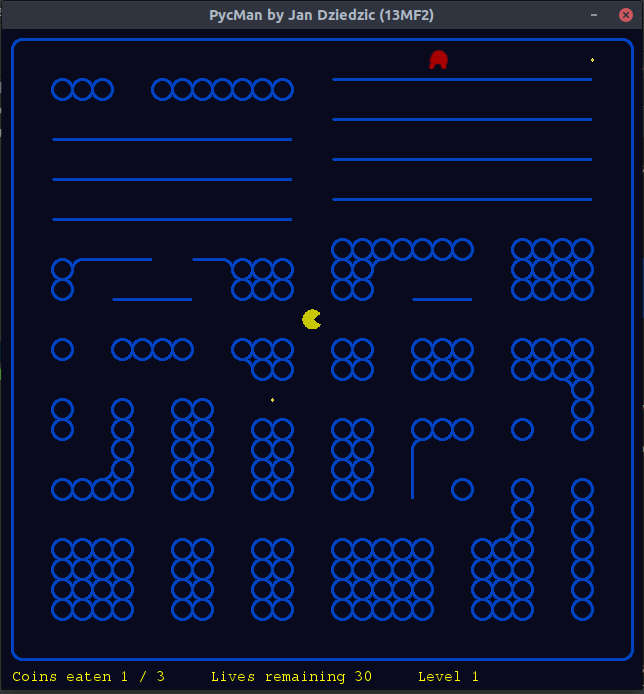
\includegraphics[width=350pt]{images/window-in-ubuntu}\\
				\caption{Game window rendered in Ubuntu Gnome graphical environment.}
			\end{img}
			
			\dsubsection{Board}
				As each level has a different layout so look of the board may vary. Please refer to Figure \ref{example_board} for an example of such board.
				\begin{img}
					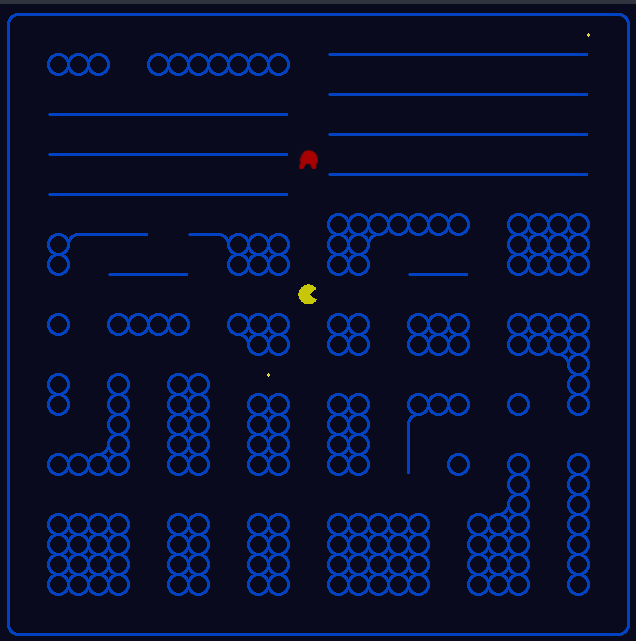
\includegraphics[width=350pt]{images/board_example}\\
					\caption{Example board. Walls, empty tiles, the player, coins and a red ghost are visible}
					\label{example_board}
				\end{img}
				General idea is that all border tiles of each level (tile system explained later) have to be walls, which creates a nice, outer border of the board with rounded edges.
			\dsubsection{Counters}
				Directly below the board, counters are located, these provide information on:
				\begin{enumerate}
					\item
						Number of coins eaten
					\item
						Number of coins that are required to be consumed before progressing to the next level
					\item
						Number of player lives
					\item
						Current level number
				\end{enumerate}
				\begin{img}
					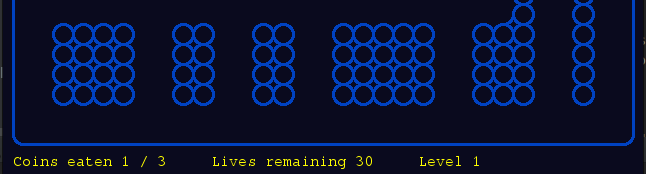
\includegraphics[width=350pt]{images/counter_example}\\
					\caption{Example set of counters with part of the board included for position reference.}
				\end{img}
				Every time the player eats a 'coin' the first counter increases. Throughout the level, this counter cannot decrease as even upon player's death, the already-eaten coins don't respawn.
				
				Number of coins required to progress is constant through the level but may differ between levels. It is worth mentioning that as every coin must be eaten to progress, this acts as a total number of coins allocated in each level map. Coin placing algorithm described later in this document also proves that it equals to $32^2-\#_{wall\_tiles}-\#_{empty\_ tiles}$.
				
				Each time a player comes in contact with a ghost(defined later in this document) a life is subtracted and every time the player eats a heart eatable, a life is added.
				
				Level number increases from 1 (easiest level) up to ten (hardest level), as player advances through the levels.
		\section{Grid layout}
			Pygame provides a sprite attribute of its location but as I have decided to use a window of over 500x500px of size, its pixel-accurate positioning would be an overkill and could make programming harder as well as require more processing power to (later mentioned) pathfinding algorithms.
			Due to this I have turned to the original PacMan solution (as read in Reference \ref{stronaopacmanie}), the grid system.
			\begin{img}
				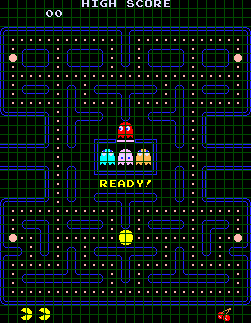
\includegraphics[width=350pt]{images/oryginal_pacman_grid}\\
				\caption{Original Pac-Man with grid layout depicted. Source: Reference \ref{stronaopacmanie}}
			\end{img}
			The PycMan board was initially made as a 64x64 grid, where each piece, namely a tile, was either a wall or a space a sprite may move on. First levels were designed this way and I found the level design a really hard task. Only later I have noticed that the grid of the original PacMan was barely $\dfrac{1}{4}^{\text{th}}$ of the size I have used, my board was just to big for a pleasant gameplay.
			
			As I wanted the board to be square I have decided to move to 32x32 grid. Some testing later I have decided that this size not only nicely divides by 2 making perfectly symmetrical or even fractal levels possible to make but also is actually quite the one most similar in terms of number of tiles to the one the original PacMan had (for square boards).
			\begin{img}
				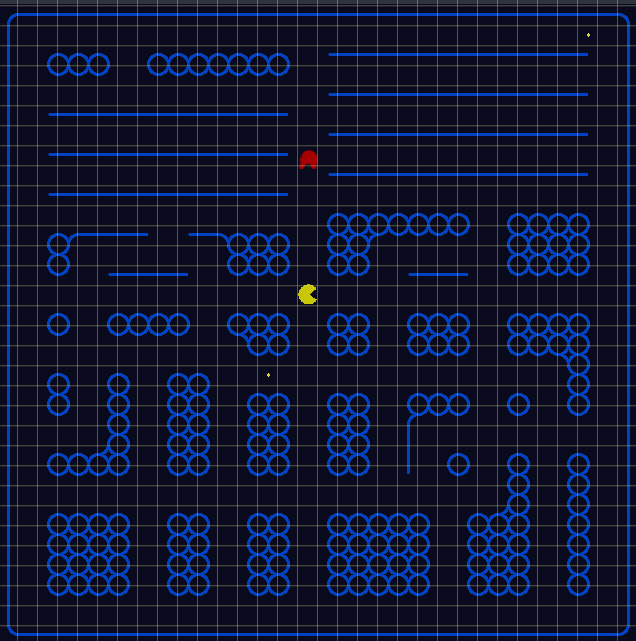
\includegraphics[width=350pt]{images/board_grid}\\
				\caption{Example of a board with a grid applied (note that the grid was added just for demonstrative purposes and in not a part of the game.)}
			\end{img}
			The following section describes types of different tiles used throughout the game.
		\section{Types of tiles}
			\dsubsection{Walls}
				As wall tiles have to connect with neighboring (common edge) tiles, they need to be represented by different graphics depending on their surroundings. 
				There is a total of 15 graphics depicted below. The system of numbering them is really intuitive, it consists of four digits each of which is either zero or one
				
				\begin{img}
					\frame{
\includegraphics{images/w0001}}\\
					\caption{Wall 0001}
				\end{img}
				\begin{img}
					\frame{
\includegraphics{images/w0010}}\\
					\caption{Wall 0010}
				\end{img}
				\begin{img}
					\frame{
\includegraphics{images/w0011}}\\
					\caption{Wall 0011}
				\end{img}
				\begin{img}
					\frame{
\includegraphics{images/w0100}}\\
					\caption{Wall 0100}
				\end{img}
				\begin{img}
					\frame{
\includegraphics{images/w0101}}\\
					\caption{Wall 0101}
				\end{img}
				\begin{img}
					\frame{
\includegraphics{images/w0110}}\\
					\caption{Wall 0110}
				\end{img}
				\begin{img}
					\frame{
\includegraphics{images/w0111}}\\
					\caption{Wall 0111}
				\end{img}
				\begin{img}
					\frame{
\includegraphics{images/w1001}}\\
					\caption{Wall 1001}
				\end{img}
				\begin{img}
					\frame{
\includegraphics{images/w1010}}\\
					\caption{Wall 1010}
				\end{img}
				\begin{img}
					\frame{
\includegraphics{images/w1011}}\\
					\caption{Wall 1011}
				\end{img}
				\begin{img}
					\frame{
\includegraphics{images/w1100}}\\
					\caption{Wall 1100}
				\end{img}
				\begin{img}
					\frame{
\includegraphics{images/w1101}}\\
					\caption{Wall 1101}
				\end{img}
				\begin{img}
					\frame{
\includegraphics{images/w1110}}\\
					\caption{Wall 1110}
				\end{img}
				\begin{img}
					\frame{
\includegraphics{images/w1111}}\\
					\caption{Wall 1111}
				\end{img}
				
			
				The first bit represents whether connection is to be made on the right, second whether on the top, third whether on the left and fourth whether on the bottom. As wall 0000 would be very small and hard to maneuver around for user, drawing of such is unsupported. I have actually tested moving around such and even my manual and keyboard skills are relatively good, I found it hard to move around such.
				
				Algorithm deciding which type of wall is presented below:
				\label{walltypecheck}
				\begin{lstlisting} [language=Python]
def walltypecheck(location):
	r = t = l = b = 0
	if location[0] != 0:
		if level[location[0]-1][location[1]] == wall:
			l = 1
	if location[0] != 31:
		if level[location[0]+1][location[1]] == wall:
			r = 1
	if location[1] != 0:
		if level[location[0]][location[1]-1] == wall:
		t = 1
	if location[1] != 31:
		if level[location[0]][location[1]+1] == wall:
			b = 1
	return str(r) + str(t) + str(l) + str(b)
				\end{lstlisting}
				For reference of how level data is stored see section \ref{Levels}.
				This algorithm returns type of wall that would fit in the spot location provided as an argument while calling the function. Output format is a string corresponding with wall names described above.
			\dsubsection{Player}
				Player is represented by an iconic PacMan figure of my own design (to avoid direct copying of work of others). The tile rotates depending on the direction of player's movement so that the 'mouth' is always facing forward. Color has been slightly darkened as I find this design a little bit nicer than the original.  
				\begin{img}
					
\includegraphics{images/player}\\
				\caption{Player sprite}
				\end{img}
			\dsubsection{Ghosts}
				There are three types of ghosts in the game, red, green and blue. They are similar in design, though they behavior is different. (described later)
				 \begin{img}
				 	
\includegraphics{images/redghost}\\
				 	\caption{Red ghost sprite}
				 \end{img}
				  \begin{img}
				 	
\includegraphics{images/greenghost}\\
				 	\caption{Green ghost sprite}
				 \end{img}
				 \begin{img}
				 	
\includegraphics{images/blueghost}\\
				 	\caption{Blue ghost sprite}
				 \end{img}
			\dsubsection{Eatables}
				\subsubsection{Coins}
					Coin spawning works a little bit different than spawning other tiles, which is described later. They actually appear in every tile \textbf{not} designated as 'wall', 'heart' or 'empty'. They are static and their sprites are killed when player enters their tile resulting in coins-eaten counter value increasing.
					\begin{img}
						
\includegraphics{images/coin}\\
						\caption{Coin graphics}
					\end{img}
				\subsubsection{Hearts}
					Hearts are similar to coins in terms of being eaten, but they spawn in designated places and their consumption increases lives counter.
					%TODO: Heart graphics
			\dsubsection{Empty tiles}
				These tiles are actually not drawn. They only act as an abstract concept to hold information that coin is not to be drawn on this particular grid tile. Player and ghost can move through this tile. For user these appear as plain dark blue space - the color of the background.
		\section{Levels}
		\label{Levels}
			\dsubsection{Permanent storing}
				It took me a while to actually figure out how to store level blueprints. The container had to be a 32x32 matrix of values. Python lists of lists of variables would actually be the most efficient way to store types of tiles on each position in the grid. I have actually tried this approach back when my original board was still 64x64 tiles and it didn't take me 10 tiles of brackets and commas to figure out, that maybe this approach is most efficient for storing, but it is absolutely to slow to prepare the level of 4096 tiles. I have decided that I need an editing software for these grids. Then I understood that my levels, grids of values are actually bitmaps. I have prepared an exemplar of a level in GIMP and using my previous experience with Pillow module I have prepared a script to load these bitmaps to my Python program. It all took less time that it would take to fill $\dfrac{1}{10}^{\text{th}}$ of that list of lists of values manually.
				\begin{img}
					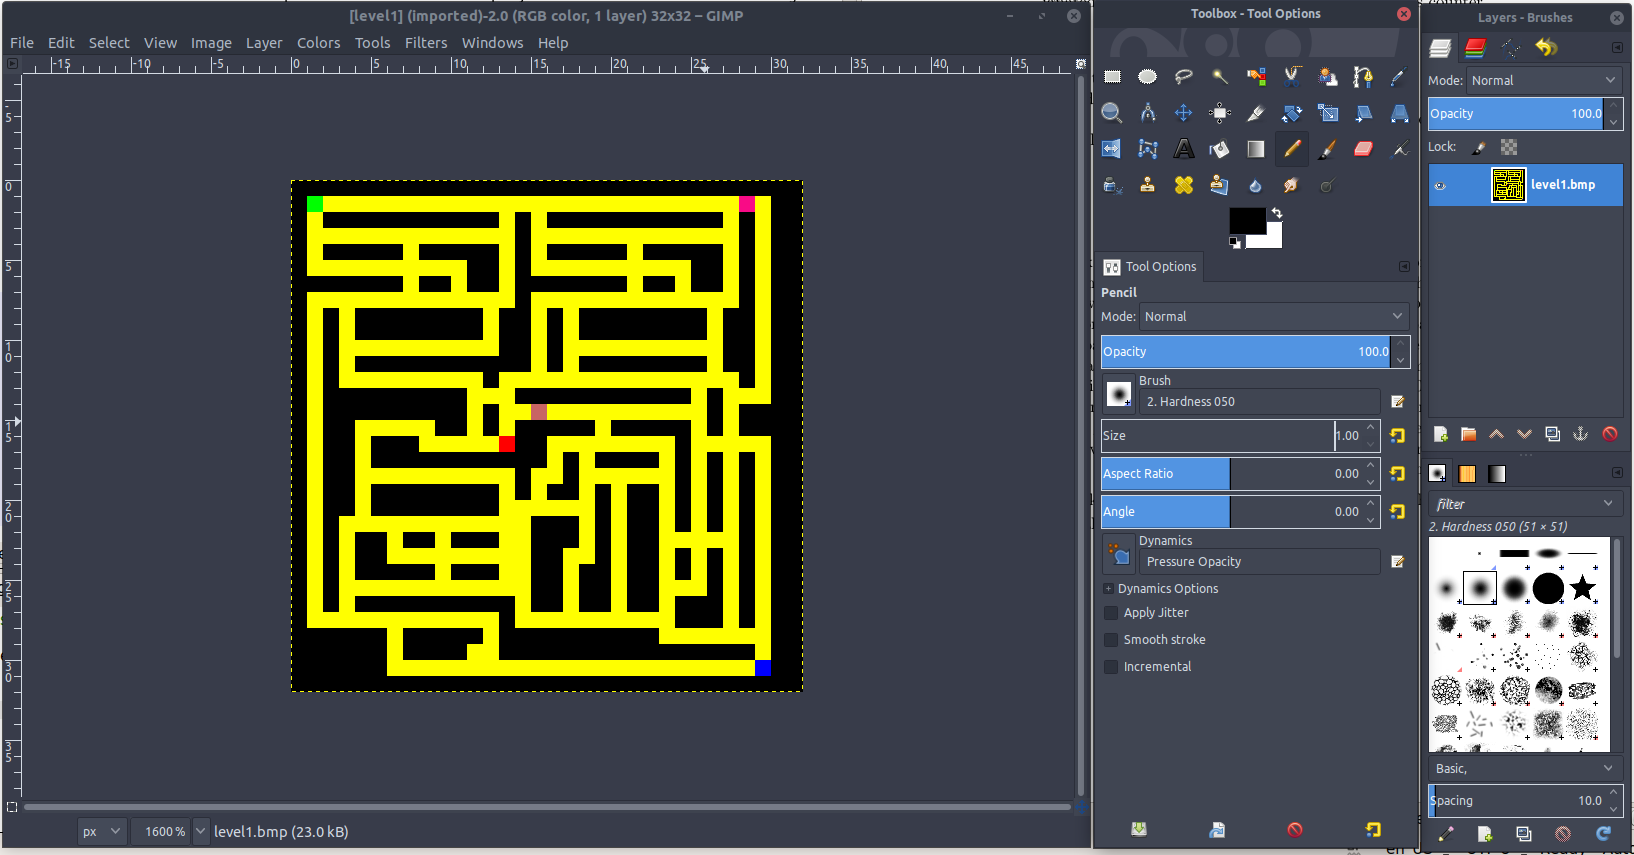
\includegraphics[width=350pt]{images/gimp_level_editing}\\
					\caption{An exemplar of a level being edited in the GIMP software}
					\label{gimplevel}
				\end{img}
				Each tile has its representation in a particular color in RGB notation:\\ \\
				\begin{tabular}{| l | r |}
					\hline 
					Empty tile & (255, 255, 255) \\ \hline
					Wall & (0, 0, 0) \\ \hline
					Coin & (255, 255, 0) \\ \hline
					Player & (255, 0, 0) \\ \hline
					Red Ghost & (200, 100, 100) \\ \hline
					Green Ghost & (0, 255, 0) \\ \hline
					Blue Ghost & (0, 0, 255) \\ 
					%TODO: heart color
					\hline
				\end{tabular}
			\dsubsection{Storing while in game}
				Do you remember my first concept for the most optimal storage of levels mentioned earlier? Well, that didn't work for storing levels as files... But in game while loaded in RAM - works like a charm. List of lists of integers, just like that:\\
				\noindent
				\begin{center}
					\begin{small}
					 [[1, 1, 1, 1, 1, 1, 1, 1, 1, 1, 1, 1, 1, 1, 1, 1, 1, 1, 1, 1, 1, 1, 1, 1, 1, 1, 1, 1, 1, 1, 1, 1], \\ [0pt] 
					 [1, 0, 0, 0, 0, 0, 0, 0, 0, 0, 0, 0, 0, 0, 0, 0, 0, 0, 0, 0, 0, 0, 0, 0, 0, 0, 0, 0, 0, 0, 0, 1], \\ [0pt] 
					 [1, 0, 1, 1, 0, 1, 0, 1, 0, 1, 0, 1, 1, 1, 0, 1, 1, 0, 1, 1, 1, 0, 1, 1, 0, 1, 1, 1, 1, 1, 0, 1], \\ [0pt] 
					 [1, 0, 1, 1, 0, 1, 0, 1, 0, 1, 0, 1, 1, 1, 0, 1, 1, 0, 1, 1, 1, 0, 1, 1, 0, 1, 1, 1, 1, 1, 0, 1], \\ [0pt] 
					 [1, 0, 1, 1, 0, 1, 0, 1, 0, 1, 0, 1, 0, 0, 0, 0, 0, 0, 0, 0, 0, 0, 1, 1, 0, 1, 1, 1, 1, 1, 0, 1], \\ [0pt] 
					 [1, 0, 1, 1, 0, 1, 0, 1, 0, 1, 0, 1, 0, 1, 0, 1, 1, 0, 1, 1, 1, 1, 1, 1, 0, 1, 1, 1, 1, 1, 0, 1], \\ [0pt] 
					 [1, 0, 0, 0, 0, 1, 0, 1, 0, 1, 0, 1, 0, 1, 0, 1, 1, 0, 1, 1, 1, 1, 1, 1, 0, 1, 1, 1, 1, 1, 0, 1], \\ [0pt] 
					 [1, 0, 1, 1, 0, 1, 0, 1, 0, 1, 0, 1, 0, 1, 0, 1, 1, 0, 0, 0, 0, 0, 0, 0, 0, 0, 0, 0, 0, 0, 0, 1], \\ [0pt] 
					 [1, 0, 1, 1, 0, 1, 0, 1, 0, 1, 0, 0, 0, 1, 0, 1, 1, 0, 1, 1, 1, 1, 1, 1, 0, 1, 1, 1, 1, 1, 0, 1], \\ [0pt] 
					 [1, 0, 1, 1, 0, 1, 0, 1, 0, 1, 0, 1, 0, 1, 0, 1, 1, 0, 1, 1, 1, 1, 1, 1, 0, 1, 1, 1, 1, 1, 0, 1], \\ [0pt] 
					 [1, 0, 1, 1, 0, 1, 0, 1, 0, 1, 0, 1, 0, 0, 0, 0, 0, 0, 1, 1, 1, 1, 1, 1, 0, 1, 1, 1, 1, 1, 0, 1], \\ [0pt] 
					 [1, 0, 1, 1, 0, 1, 0, 1, 0, 1, 0, 1, 1, 1, 0, 1, 1, 0, 0, 0, 0, 0, 0, 0, 0, 0, 0, 0, 0, 0, 0, 1], \\ [0pt] 
					 [1, 0, 1, 1, 0, 1, 0, 1, 0, 1, 0, 1, 1, 1, 0, 1, 1, 1, 0, 1, 1, 1, 1, 1, 0, 1, 1, 1, 1, 1, 0, 1], \\ [0pt] 
					 [1, 0, 1, 1, 0, 1, 0, 1, 0, 1, 0, 1, 1, 1, 0, 1, 1, 1, 2, 1, 1, 1, 1, 1, 0, 1, 1, 1, 1, 1, 0, 1], \\ [0pt] 
					 [1, 0, 1, 1, 0, 1, 0, 1, 0, 1, 0, 1, 1, 1, 0, 1, 1, 1, 0, 1, 1, 1, 1, 1, 0, 1, 1, 1, 1, 1, 0, 1], \\ [0pt] 
					 [1, 0, 0, 0, 0, 0, 0, 0, 0, 0, 0, 0, 0, 0, 3, 0, 0, 0, 0, 0, 0, 0, 0, 0, 0, 0, 0, 0, 0, 0, 0, 1], \\ [0pt] 
					 [1, 0, 1, 0, 1, 0, 1, 0, 1, 0, 1, 1, 1, 1, 0, 1, 1, 1, 0, 1, 1, 1, 1, 1, 0, 1, 1, 1, 1, 1, 0, 1], \\ [0pt] 
					 [1, 0, 1, 0, 1, 0, 1, 0, 1, 0, 1, 1, 1, 1, 0, 1, 1, 1, 0, 1, 1, 1, 1, 1, 0, 1, 1, 1, 1, 1, 0, 1], \\ [0pt] 
					 [1, 0, 1, 0, 1, 0, 1, 0, 1, 0, 1, 1, 1, 1, 0, 1, 1, 1, 0, 1, 1, 1, 1, 1, 0, 1, 1, 1, 1, 1, 0, 1], \\ [0pt] 
					 [1, 0, 1, 0, 1, 0, 1, 0, 1, 0, 1, 1, 0, 0, 0, 0, 0, 0, 0, 0, 0, 0, 0, 0, 0, 1, 1, 1, 1, 1, 0, 1], \\ [0pt] 
					 [1, 0, 1, 0, 1, 0, 1, 0, 1, 0, 1, 1, 0, 1, 0, 1, 1, 1, 0, 1, 1, 1, 1, 1, 0, 1, 1, 1, 1, 1, 0, 1], \\ [0pt] 
					 [1, 0, 1, 0, 1, 0, 1, 0, 1, 0, 1, 1, 0, 1, 0, 1, 1, 1, 0, 1, 1, 0, 0, 0, 0, 1, 1, 1, 1, 1, 0, 1], \\ [0pt] 
					 [1, 0, 1, 0, 1, 0, 1, 0, 1, 0, 1, 1, 0, 1, 0, 1, 1, 1, 0, 1, 1, 0, 1, 1, 0, 0, 0, 0, 0, 0, 0, 1], \\ [0pt] 
					 [1, 0, 1, 0, 1, 0, 1, 0, 1, 0, 1, 1, 0, 1, 0, 1, 1, 1, 0, 1, 1, 0, 1, 1, 0, 1, 1, 1, 1, 1, 0, 1], \\ [0pt] 
					 [1, 0, 1, 0, 1, 0, 1, 0, 1, 0, 0, 0, 0, 0, 0, 0, 0, 0, 0, 0, 0, 0, 0, 0, 0, 1, 1, 1, 1, 1, 0, 1], \\ [0pt] 
					 [1, 0, 1, 0, 1, 0, 1, 0, 1, 0, 1, 1, 1, 1, 0, 1, 1, 1, 0, 1, 1, 0, 1, 1, 1, 1, 1, 1, 1, 1, 0, 1], \\ [0pt] 
					 [1, 0, 1, 0, 1, 0, 1, 0, 1, 0, 1, 1, 1, 1, 0, 1, 1, 1, 0, 1, 1, 0, 1, 1, 1, 1, 1, 1, 1, 1, 0, 1], \\ [0pt] 
					 [1, 0, 1, 0, 1, 0, 1, 0, 1, 0, 1, 1, 1, 1, 0, 1, 1, 1, 0, 0, 0, 0, 0, 0, 0, 0, 0, 0, 0, 0, 0, 1], \\ [0pt] 
					 [1, 0, 1, 0, 1, 0, 1, 0, 1, 0, 1, 1, 1, 1, 0, 1, 1, 1, 1, 1, 1, 0, 1, 1, 1, 1, 1, 1, 1, 1, 0, 1], \\ [0pt] 
					 [1, 4, 1, 0, 1, 0, 1, 0, 1, 0, 1, 1, 1, 1, 0, 1, 1, 1, 1, 1, 1, 0, 1, 1, 1, 1, 1, 1, 1, 1, 0, 1], \\ [0pt] 
					 [1, 0, 0, 0, 0, 0, 0, 0, 0, 0, 0, 0, 0, 0, 0, 0, 0, 0, 0, 0, 0, 0, 0, 0, 0, 0, 0, 0, 0, 0, 0, 1], \\ [0pt] 
					 [1, 1, 1, 1, 1, 1, 1, 1, 1, 1, 1, 1, 1, 1, 1, 1, 1, 1, 1, 1, 1, 1, 1, 1, 1, 1, 1, 1, 1, 1, 1, 1]] \\ [0pt] 
				\end{small}
				\end{center}
				\newpage
				Where every value represents a different type of tile.\\ \\
				\begin{tabular}{| l | r |}
					\hline 
					Empty tile & 0 \\ \hline
					Wall & 1 \\ \hline
					Coin & 2 \\ \hline
					Player & 3 \\ \hline
					Red Ghost & 4 \\ \hline
					Green Ghost & 5 \\ \hline
					Blue Ghost & 6 \\ 
					%TODO: heart value
					\hline
				\end{tabular}
			\dsubsection{Interpreting}
				\begin{img}
					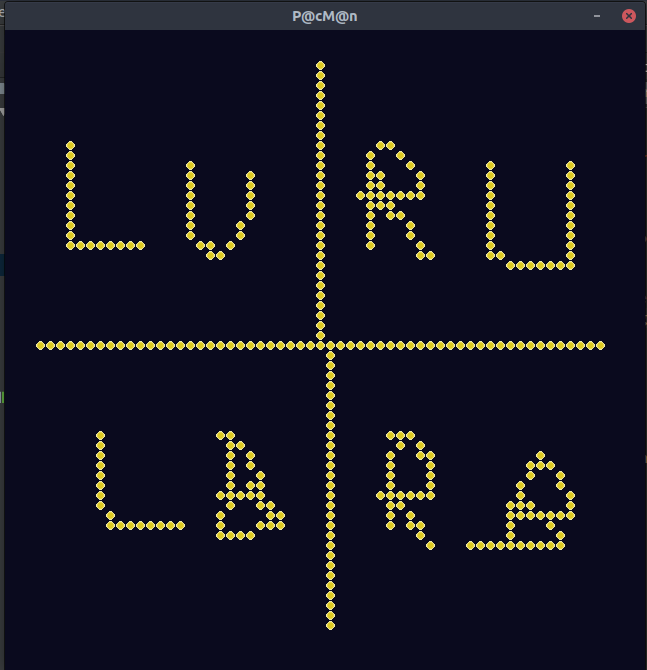
\includegraphics[width=350pt]{images/aligning-level}\\
					\caption{First tests of interpretation of level files. Note that coins are formed into letters LU, RU, LB, RB as in words Left, Right, Upper, Bottom to load the tiles in the right orientation. Old 64x64 grid is used.}
				\end{img}
				These tables are then interpreted for program to know where to place which sprites, therefore the following algorithm is used:\\
				\begin{lstlisting} [language=Python]
if level[column][row] = wall
	spawn wall at location column, row
elif level[column][row] = player
	spawn player at location column, row
elif level[column][row] = coin
	spawn coin at location column, row
elif level[column][row] = ghost
	gtype = check ghost color
	spawn ghost of color gtype at location column, row
elif level[column][row] = heart
	spawn heart at location column, row
				\end{lstlisting}
			\dsubsection{Designing the levels}
				Process of level design is quite easy and only limitation one needs to remember is that all coin - having tiles must be accessible by a player - not surrounded by a wall. The rest is just a subjective approach to the difficulty. As not all ghosts have to be used, the first few levels have one or two ghosts at most, making them easier. Through alpha testing I have noticed that long passages are traps, as one ghost may approach player from one side and other from the other and there is nowhere to hide. Also it's easier for ghosts to navigate through complex maze and these might be finger-tangling even for advanced players.
				See Figure \ref{gimplevel} for a screenshot of a design process.
			\dsubsection{User-defined levels}
				As levels can be created using a very basic bitmap editing software, user might actually add their own levels. And use them instead of the built-in ones.
			\dsubsection{Progressing to the next level}
				When player eats all coins, they advance to the next level. At this stage a message screen (described later) appears and all level - loading procedures are called. Also counters of coins eaten and total are reset at this point.
				
				If the level completed was the last level, a congratulations screen is displayed and the game eventually quits.
				
				See Section \ref{typesofscreens} for reference on messages signaling level change and completing the game.
		\section{Gameplay scheme}
			The game works on a concept of a loop, that (when run on a sufficiently fast machine) executes 60 times per second. During that time multiple  conditions are checked and different procedures are called.
			\dsubsection{Introduction to the concept of time segments}
				\label{timesegments}
				\begin{img}
					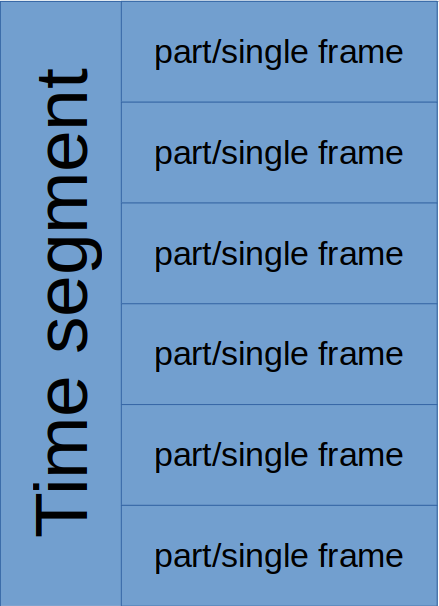
\includegraphics[width=180pt]{images/segment-part-relation}\\
					\caption{Scheme depicting relation between a time segment and parts}
					\label{segment-part-relation}
				\end{img}
				It's actually not required to compute some values every each of these 60 loop repetitions per second. An example - ghost moves $\dfrac{1}{10}^{\text{th}}$ of a tile in that time, it still can't turn so its path to the unchanged player location will remain the same. That's why I have introduced "Time segments". These are discrete representations of time period which is required for a ghost or a player to move a length of one tile. As ghost are slower, they have 5 of these in a second and player has 6. 
				\label{part_definition}
				
				Whilst processing single frames is still needed, these were called parts, whilst introducing 'part' variable determining which part of time segment is currently executed. See Figure \ref{segment-part-relation} for reference.
			\dsubsection{Player movement}
				Every player's time segment the following code is called:
				\begin{lstlisting} [language=Python]
# ----- checking pressed keys -----
keys = pygame.key.get_pressed()
# ----- wall collision check -----
surroundings = walltypecheck(player.location)
				\end{lstlisting}
				It's worth noting that I have reused walltypecheck to look for surroundings of the player for walls. See section \ref{walltypecheck} for reference on how this algorithm works.
				
				Then check is performed whether player's move is legit (wall does not obstruct it).
				\begin{lstlisting}[language=Python]
if keys[pygame.K_LEFT] and surroundings[2] == '0':
	player.move('left', player_part)
elif keys[pygame.K_RIGHT] and surroundings[0] == '0':
	player.move('right', player_part)
elif keys[pygame.K_UP] and surroundings[1] == '0':
	player.move('up', player_part)
elif keys[pygame.K_DOWN] and surroundings[3] == '0':
	player.move('down', player_part)
				\end{lstlisting}
				Please note usage of the player\_part variable. It is the value of frames that have passed since last player segment begun (as described in Section \ref{timesegments}). It's useful to determine whether a new time segment is to be started and for player's moving routine to know at which part of tile it should position player's sprite inducing a fluency of movement.
				\begin{img}
					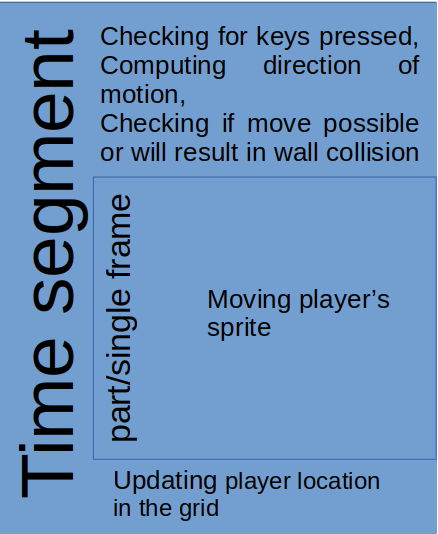
\includegraphics[width=180pt]{images/movement-diagram}\\
					\caption{Diagram showing how tasks are executed either once per time segment or once per part}
				\end{img}
			\dsubsection{Ghost movement}
				Ghost movement is a far more complex algorithm than player's movement though it uses same concept of time segments.
				
				As mentioned in Success Criteria \ref{smarterghosts}, I wanted the ghosts to be more intelligent than the originals. I have read (Reference \ref{stronaopacmanie}) that the original algorithm is really primitive. It checks from which of surrounding tiles ghost will be straight-line closest to the player and moves there.
				\subsubsection{The graph}
					First idea of mine was to make the ghost actually pick the shortest path to the player. That would have to involve implementation of a graph and a pathfinding algorithm.
					
					As I already had my level-keeping structure in place I have decided to use a similar one to store my graph. It is represented as a list of lists of lists of location tuples. It looks confusing so...\\
					A list (index i) of lists (index j) is used so that all nodes accessible from node of location (i, j) can be stored. Then that next list stores tuples (x, y) of locations accessible from that node.
					Object is named 'thegraph' throughout the program (as it is the only graph implementation in it). Note that it is a global object.
					
					It's obviously individual for each level and is built every time a level is loaded. Through the following routine:
					\begin{lstlisting}
def graphbuilder():
	global level, thegraph
	thegraph = [[[] for i in range(32)] for j in range(32)]
	for i in range(32):
		for j in range(32):
			if level[i][j] != wall:
				location = [i, j]
				if location[0] != 0:
					if level[location[0] - 1][location[1]] != 	wall:
						thegraph[location[0]][location[1]] += [[location[0] - 1, location[1]]]
				if location[0] != 31:
					if level[location[0] + 1][location[1]] != wall:
						thegraph[location[0]][location[1]] += [[location[0] + 1, location[1]]]
				if location[1] != 0:
					if level[location[0]][location[1] - 1] != wall:
						thegraph[location[0]][location[1]] += [[location[0], location[1] - 1]]
				if location[1] != 31:
					if level[location[0]][location[1] + 1] != wall:
						thegraph[location[0]][location[1]] += [[location[0], location[1] + 1]]
					\end{lstlisting}
				\subsubsection{Pathfinding}
					This part I found actually the hardest. All my previous experience with graphs and pathfinding was actually from old times when my favorite language was C++. Apparently when I switched to Python, my rusty knowledge on the topic had to be refreshed. My first approach (a stupid one) was to use DFS search to check all possible paths and decide which one to use.
					\begin{img}
						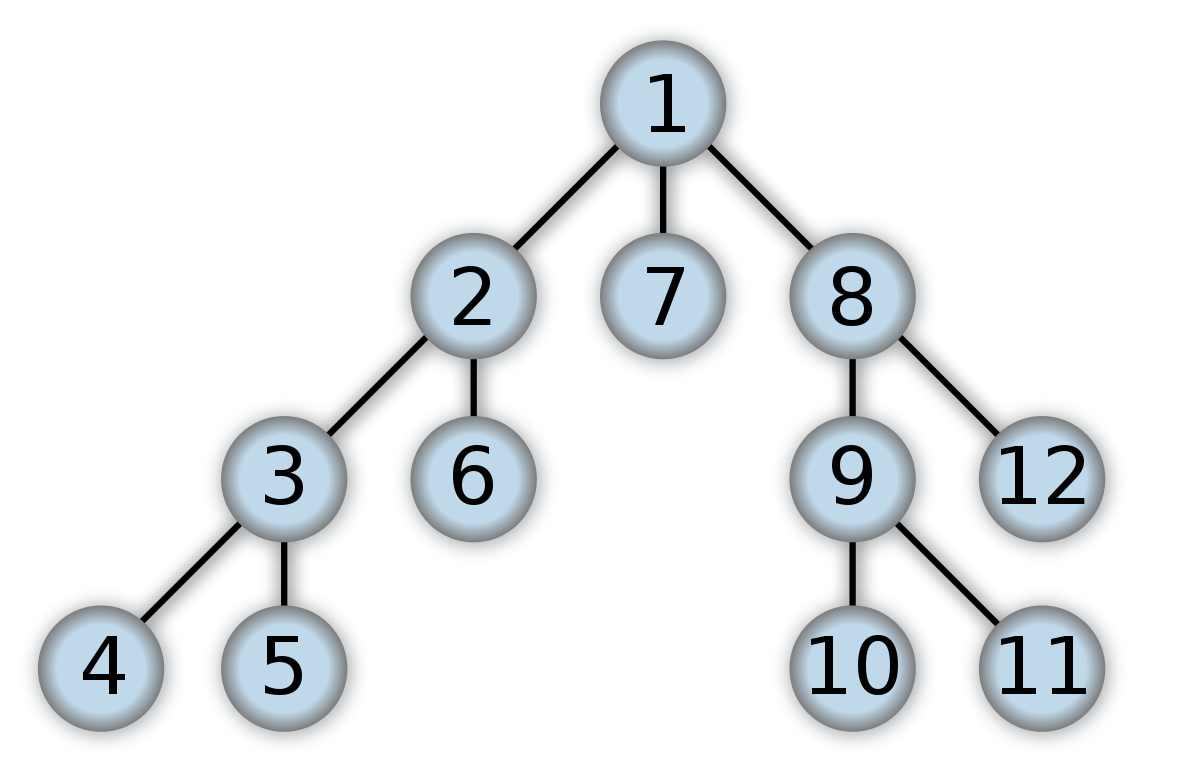
\includegraphics[width=350pt]{images/dfs-diagram}\\
						\caption{Diagram showing order of nodes visits starting from node 1 using DFS algorithm Source: wikipedia.org}
					\end{img}
					It was a rather simple recursion.
					\begin{lstlisting} [language=Python]
def findpath(start, end, path):
	append start to path
	if start == end:
		return path
	else:
		for neighbour in neighbours(start): # neighbours easily obtained from thegraph
			findpath(neighbour, end, path)
					\end{lstlisting}
					That was stupid and very slow, as I have noticed that my graph is not actually a tree and paths may have cycles, this process never actually worked.
					
					And then I realized that a more appropriate solution was to use BFS and implement whether a new node was actually visited before.
					
					\begin{img}
						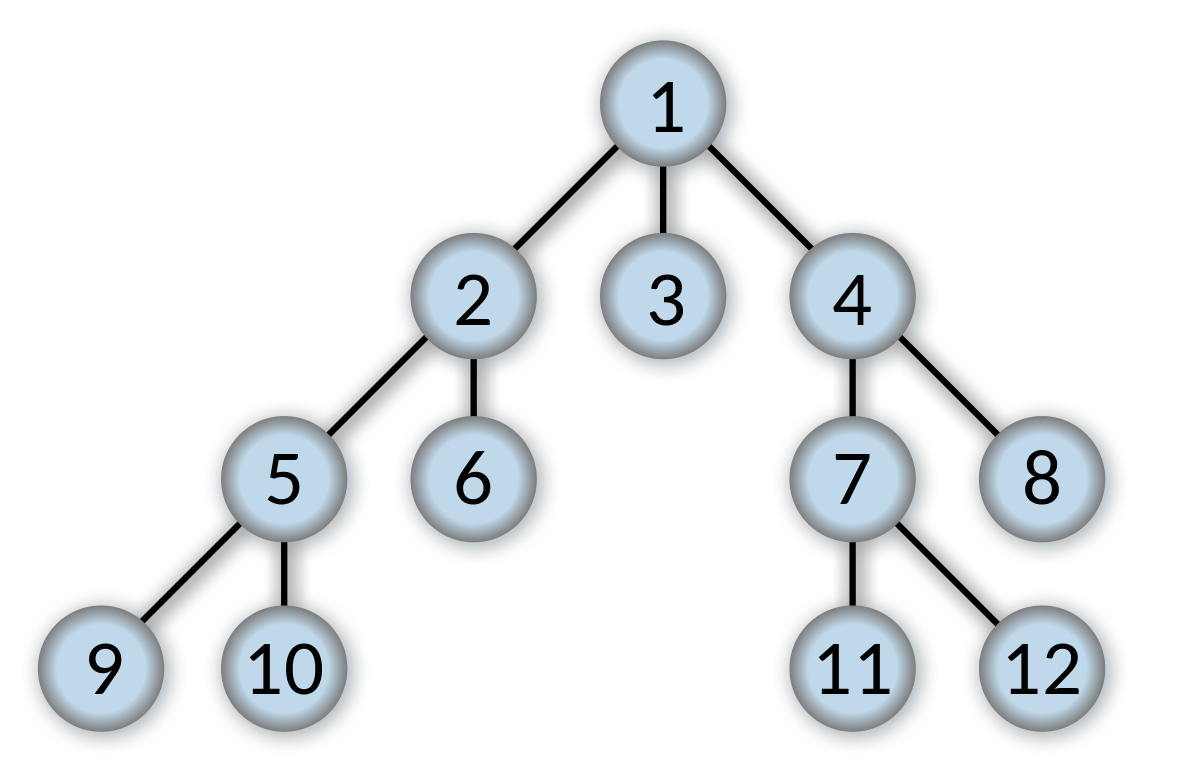
\includegraphics[width=350pt]{images/bfs-diagram}\\
						\caption{Diagram showing order of nodes visits starting from node 1 using BFS algorithm Source: wikipedia.org}
					\end{img}
					
					I also dropped recursion as advised by online forums... Maybe recursion is a way in C++ but in Python it apparently is really slow. Also my own testing of recursive approach sometimes lead to stack overflows, which disqualified this method completely.
					
					A queue of nodes to visit was implemented and new algorithm came to life. It was fast but its output of a complete path to player was actually an overkill - why would I need it if it will become obsolete in the next time segment when player location changes?
					
					The next iteration actually begins BFSing from the player, until it finds any of the tiles surrounding the ghost. It then returns location of such tile - next tile ghost has to move to.
					
					\begin{lstlisting}[language=Python]
def find_next_move(start, end, forbidden):
	visited = []
	queue = []
	neighbours = thegraph[start[0]][start[1]].copy()
	queue.append([end[0], end[1]])
	visited.append(end)
	for point in queue:
		if point not in visited:
			visited.append(point)
		if point in neighbours:
			return point
		for node in thegraph[point[0]][point[1]]:
			if node not in visited:
				queue.append(node)
					\end{lstlisting}
					
					As this approach worked, I was satisfied with its speed and overall performance. Then in alpha testing I found a strange occurrence I haven't noticed in the original PacMan - ghosts could reverse.
					
					I didn't like it, so the algorithm had to exclude ghost's previous location from its neighboring tiles. The next version looked like this:
					\begin{lstlisting}[language=Python]
def find_next_move(start, end, forbidden):
    visited = []
    queue = []
    neighbours = thegraph[start[0]][start[1]].copy()
    neighbours.remove([forbidden[0], forbidden[1]])
    queue.append([end[0], end[1]])
    visited.append(end)
    for point in queue:
        if point not in visited:
            visited.append(point)
        if point in neighbours:
            return point
    for node in thegraph[point[0]][point[1]]:
        if node not in visited and node != [forbidden[0], forbidden[1]]:
    queue.append(node)
					\end{lstlisting}
				\subsubsection{Difference between ghosts}
					As I have generated some levels and started testing, I found out that if two ghost share location, they effectively become one as their optimal paths will be the same and they will always move the same way. That of course wasn't the effect I wanted, I had to figure out how to make the ghosts behave different. But how to make ghosts both smart and not going straight for the player? Internet for the win, meme pages came with help.
					\begin{img}
						
\includegraphics[width=350pt]{images/trap}\\
						\caption{Popular meme. Source: pinterest.com}
						\label{trap}
					\end{img}
					Now enlightened by a piece of digital artwork originating from Star Wars (see Figure \ref{trap}), I decided that my ghosts have to behave like they were to surround the player. How to achieve such effect? I turned to the original PacMan solution - not moving to the exact tile the player occupies. A decision was made to leave the red ghost originally smart while blue and green ghosts were to move to tiles shifted by (-2, -2) and (2, 2) vectors from the player. The result was amazing, ghosts seemed to move separately while away from the player, when they approach it, I had a sense that this is not what I programmed, \textbf{They hunt in a pack!} I had an authentic experience of ghosts setting a trap, green and blue were blocking my exit routes, when red went straight for me.
					
					But it sometimes crashed, I wondered what was the case and then I found out that the ghosts were actually trying to go to a tile, which is either a wall (inaccessible) or outside the board (object level was referenced with an invalid index, either negative or exceeding it's length). I had to write a piece of algorithm to look for a nearest tile that is actually not wall.
					
					\begin{lstlisting} [language=Python]
def find_nearest_not_wall(point):
    if point[0] > 31:
        point[0] = 31
    if point[0] < 0:
        point[0] = 0
    if point[1] > 31:
        point[1] = 31
    if point[1] < 0:
        point[1] = 0
    radius = 1
    if level[point[0]][point[1]] != wall:
        return point
    while True:
        for i in range(point[0]-radius, point[0]+radius):
            for j in range(point[1]-radius, point[1]+radius):
                try:
                    if level[i][j] != wall:
                        return [i, j]
                except IndexError:
                    pass
        radius += 1
					\end{lstlisting}
					It first moves the point to the nearest one on the board (lines 2 to 9). Then it checks whether such point is a wall, if not, returns it (lines 11 and 12). If it was a wall it starts searching surroundings of such point in a fixed radius, starting from 1. First point it finds not to be wall is then returned.
					
					Later it had to be implemented in the pathfinding algorithm, which now looks like this:
					\begin{lstlisting} [language=Python]
def find_next_move(start, end, forbidden):
    visited = []
    queue = []
    end = find_nearest_not_wall(end)
    neighbours = thegraph[start[0]][start[1]].copy()
    neighbours.remove([forbidden[0], forbidden[1]])
    queue.append([end[0], end[1]])
    visited.append(end)
    for point in queue:
        if point not in visited:
            visited.append(point)
        if point in neighbours:
            return point
    for node in thegraph[point[0]][point[1]]:
        if node not in visited and node != [forbidden[0], forbidden[1]]:
    queue.append(node)
					\end{lstlisting}
					Note line 4. where final point is substituted with a one closest to it being actually accessible.
				\subsubsection{Calling pathfinding algorithm}
					Now, every ghosts' time segment (note that all ghosts share a single time segment), a new destination tile is calculated for each ghost and pathfinding is called to determine which tile should the ghost move to throughout the time segment.
					\begin{lstlisting} [language=Python]
for ghost in ghosts_list:
    if ghost.color == 'red':
        ghost.nexttile = find_next_move(ghost.location, player.location, ghost.previouslocation)
    elif ghost.color == 'blue':
        ghost.nexttile = find_next_move(ghost.location,
                                        [player.location[0] + 2,
                                         player.location[1] + 2],
                                        ghost.previouslocation)
    elif ghost.color == 'green':
        ghost.nexttile = find_next_move(ghost.location,
                                        [player.location[0] - 2,
                                         player.location[1] - 2],
                                        ghost.previouslocation)
					\end{lstlisting}
					Note how find\_next\_move function takes arguments of:
					\begin{enumerate}
						\item
							Ghost location
						\item
							Target location
						\item
							Previous ghost location - forbidden tile as ghosts can't reverse.
					\end{enumerate}
				\subsubsection{Ghosts speed}
					As I had ghosts chasing me, I have figured out that the player actually can't outrun them. And every suboptimal move of the player led to red ghost getting closer and closer. I had the smartest ghost possible, but it had an advantage of having no means of being killed. It was a too powerful opponent. I didn't want to add power-ups for the player to either become faster or to be able to frighten/kill the ghosts. Instead, as derived from the Interview (see Section \ref{interview}), I decided to make the ghosts move at $\dfrac{5}{6}^{\text{th}}$ of the player's speed. I found the gameplay to be quite optimal and actually started playing the game which at this stage was only running from the ghost. But with a stopwatch I was challenged to keep my distance from them for quite a long time. I finally knew that this is what I was aiming for.
			\dsubsection{Handling movement animation}
				This section is common for both ghosts and a player as it actually derives from the same code. As mentioned in Section \ref{part_definition}, the part part is a smaller piece of time segment. During a single part no routes are computed for ghosts, they only move from one tile to another, being able to actually be rendered in between these tiles to make the Movables (ghosts + player sprites) move fluently.
				\begin{lstlisting} [language=Python]
def move(direction,
				segmentsize,
				part):
	# handling multiple direction formats
    if direction == 'up' or direction == (0, 1):
        speed = (0, -1)
    elif direction == 'down'or direction == (0, -1):
        speed = (0, 1)
    elif direction == 'left' or direction == (-1, 0):
        speed = (-1, 0)
    elif direction == 'right' or direction == (1, 0):
        speed = (1, 0)
    part2 = (part+1) / segmentsize #as parts are numbered from 0
    #rect parameters of a Movable as implemented in pygame
    rect.x, rect.y = (location[0] + speed[0] * part2) * tile_width,
                     (location[1] + speed[1] * part2) * tile_width
    if part == segmentsize - 1:
    #if movement came to the end update location
        location = location[0] + speed[0],
                   location[1] + speed[1]
				\end{lstlisting}
				\begin{enumerate}
					\item
						Speed vector is derived from parameter 'direction' (lines 4-12)
					\item
						part2 is calculated - fraction of progress of the movement to be completed in this part (line 13)\
					\item
						Movable sprite is moved to new position (lines 14-16)
					\item
						If the actual movement came to an end and a Movable is in a center of a next tile location is updated (lines 17-20)
				\end{enumerate}
			\dsubsection{Eating}
				Eating of both coins and hearts (Eatables) was easy to implement in terms of detection, but I had to look up how to destroy eaten sprites in the pygame documentation. I found that Sprites may be killed, which seemed to be an optimal solution to that problem. Therefore every player's time segment the following routine is called.
				\begin{lstlisting} [language=python]
for eatable in eatables:
	if eatable.location == player.location:
		if eatable == heart:
			lifes += 1
		if eatable == coin:
		 coins_eaten += 1
		eatable.kill()
				\end{lstlisting}
				For every eatable is checked for occupying the same tile as player.\\
				Then if it is a heart, player gains a life,\\
				if it was a coin, coins eaten counter increases.\\
				Eatable sprite is killed.
			\dsubsection{Getting killed}
				Killing a player is fairly similar to eating... It's just checking for collision with a Ghost instead of an Eatable. It's also called every player's time segment \textbf{or} every ghosts' time segment.
				Following routine is then called:
				\begin{lstlisting} [language=python]
for ghost in ghosts:
	if ghost.location == player.location:
		lives -= 1
		if lives == 0:
			pull Game Over screen
		Respawn every Movable
		Reset parts
		Wait 5s
		Continue game
				\end{lstlisting}
				For every ghost a collision with player is checked, if such is detected, process of dying begins.\\
				Life is subtracted from lives counter.\\
				If player has no more lives the game ends.\\
				If there are more lives, all movables return to their original position (described in Section \ref{respawning})
				and part counters are reset.\\
				Game waits 5 seconds to let the user cope with the loss, and continues.
			\dsubsection{Respawning after a loss of life}
				\label{respawning}
				This is a relatively simple process of putting all Movables to their initial position and making them not preserve their speed. It can be easily described with a following code:
				\begin{lstlisting} [language=Python]
for Movable in Movables:
    Movable.location = Movable.initiallocation
    Movable.speed = (0, 0)
				\end{lstlisting}
		\section{Types of message screens}
			\label{typesofscreens}
			\dsubsection{Tutorial}
				TODO: Photo of the screen
			\dsubsection{Loss of life}
				TODO: Photo of the screen
			\dsubsection{Completing the level}
				TODO: Photo of the screen
			\dsubsection{Loosing the game}
				TODO: Photo of the screen
			\dsubsection{Completing the entire game}
				TODO: Photo of the screen
		\section{Testing}
			I have decided to use three stages of testing, namely zero, alpha ($\alpha$) and beta ($\beta$).
			\dsubsection{zero-testing}
				This stage was introduced while testing single functions and procedures implemented through the game during the development process. It consisted of mostly running code as-is while writing it using PyCharm. Sometimes I haven't even use debugger in favor of print function to enlist values of variables. This phase commenced until all modules of the game were actually prepared, despite being containing minor bugs that didn't immediately throw an error. At the end of this stage, the game was playable. 
			\dsubsection{$\alpha$-testing}
				This was the stage of extensively playing the game to see whether all functions appear to be working correctly. Note the use of word 'appear' - code wasn't actually read at this stage in look for bugs, only user experience was assessed. I have tried different approaches at playing, to make the game algorithms experience different user input. From staying perfectly still to going straight for a ghost, I have played the game.
	\chapter{References}
		\begin{enumerate}
			\item
				http://gameinternals.com/post/2072558330/understanding-pac-man-ghost-behavior
				\label{stronaopacmanie}
			\item
				https://www.pygame.org/docs
				\label{pygamedocs}
		\end{enumerate}
			
\end{document}